\documentclass{replab}
\usepackage{lipsum}

% --- Información del documento ---
\title{Práctica 1}
\author{Diego Alejandro Heredia Franco}

% Nota: Si se desea incluir más de un autor en el documento, el archivo replab.cls, en la sección "Página de título de documento", contiene líneas de código comentadas pensadas para introducir los datos desde 1 hasta 4 autores. Sin embargo, debe escogerse solo una de las cuatro secciones de código y comentar las demás para mantener la consistencia del documento.

\date{\today}
\subtitle={Propagación de Errores en Mediciones}
\email={\href{mailto:dherediaf@unal.edu.co}{\color{principaluno}\texttt{dherediaf@unal.edu.co}}}
\subject={Laboratorio Fundamentos de Mecánica}

\setlength{\columnsep}{14pt}

% --- Archivo de bibliografía ---
\addbibresource{repbib.bib}

% --- Inicio del documento ---
\begin{document}
\setlength{\parindent}{0pt}
	
	\pagestyle{fancy}
	\unspacedoperators
	
% --- Título ---

		\begin{center}
			\maketitle
			
			{\begin{tcolorbox}[colframe=white, colback=principaldos, arc=8pt]
				\textit{\textbf{Objetivos de Aprendizaje:}}

				\begin{itemize}
					\item Apreciar y comparar las características de diferentes instrumentos de medición.
					\item Aplicar conceptos y métodos de la teoría de la medición y de la teoría de errores.
				\end{itemize}

				\textbf{Objetivos Práctica:}

				\begin{itemize}
					\item Determinar el volumen y área superficial de un objeto sólido teniendo en cuenta la propagación de errores sistemáticos en su cálculo.
					\item Caracterizar la distribución de un conjunto de datos a partir de la construcción de un histograma y el cálculo de la media, desviación estándar e incertidumbre asociada.
					\item Identificar las causas y los tipos de errores presentes en la mediciones realizadas.
				\end{itemize}

				%\medskip

				%\noindent\textit{Palabras Clave:} medidas directas e indirectas, análisis estadístico, incertidumbre, calibrador Vernier, balanza.
			\end{tcolorbox}}
		\end{center}

	\selectlanguage{spanish}
	
% --- Cuerpo del reporte ---
	\section{Marco Conceptual}

	A continuación se presentan algunas preguntas que le ayudarán a contextualizarse en la teoría de propagación de errores y análisis estadísticos necesarios para el desarrollo de la práctica. Parte de las preguntas se abordaran en clase, sin embargo se recomienda consultar la referencia \cite{ardila} para profundizar.
	
	\begin{itemize}
		\item ¿Qué es una medición directa? ¿qué es una medición indirecta?
		\item ¿Cuáles son los tipos de errores experimentales?
		\item ¿Cómo se propaga la incertidumbre asociada a errores sistemáticos?
		\item ¿Qué es un histograma? ¿cuáles son sus características? y ¿cómo se construye?
		\item ¿Cómo se determina el número de clases de un histograma? Puede investigar la regla de Sturges, regla de la raíz, etc.
		\item ¿Qué es la media aritmética y cómo se calcula?
		\item ¿Qué es la desviación estándar y cómo se calcula?
	\end{itemize}


	\section{Materiales} 

	Los materiales se proporcionarán en el laboratorio: granos, calibrador Vernier y solidos en acero. En la figura (\ref{fig:vernier}) se muestra un calibrador Vernier, también conocido como píe de rey. En clase se le indicará cómo usarlo; para más información revise \cite{cita}.

	\begin{figure}[htbp]
		\centering
		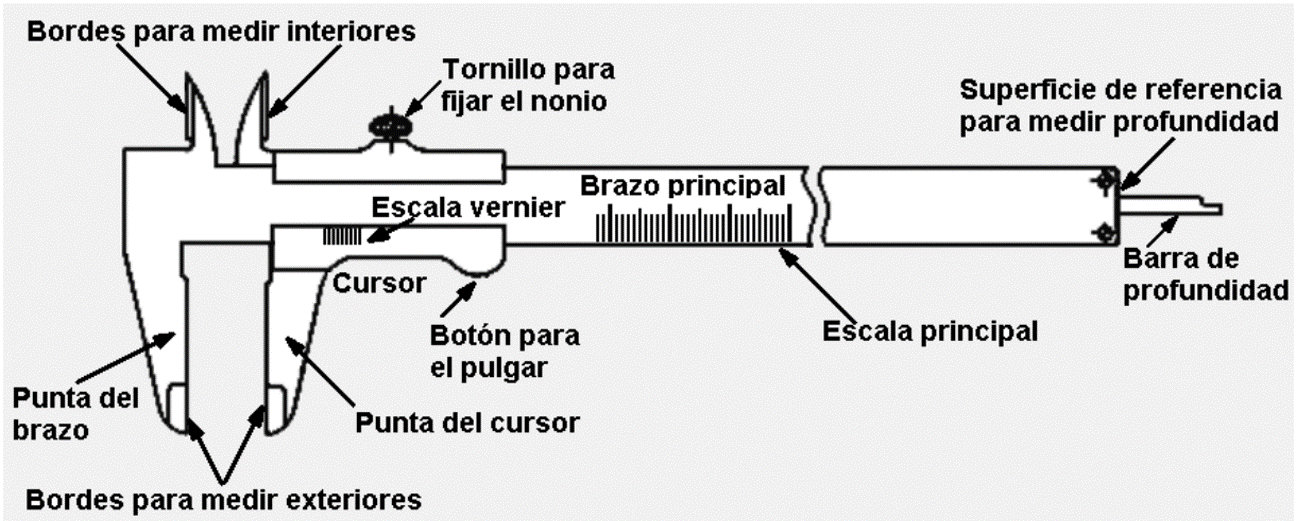
\includegraphics[width=.6\columnwidth]{imagenes/vernier1.png}
		\caption{Dibujo esquemático de un calibrador Vernier \cite{cita}.}
		\label{fig:vernier}
	\end{figure}

	\section{Experimento y Procedimiento}

	\begin{itemize}
		\item Determine la incertidumbre asociada al calibrador Vernier que se le proporcionó.
		\item Seleccione uno de los objetos dados en el laboratorio (paralelepípedo, esfera o cilindro) y tome las medidas de longitud necesarias para hallar su área superficial y volumen. Reporte estos resultados con sus respectivas incertidumbres.
		\item Posterior a ello mida el diámetro de 100 granos y con estos realice un histograma ¿cuántas clases usará? ¿obtiene una distribución normal? (es suficiente que muestre el histograma y de manera cualitativa haga su afirmación). Halle el valor promedio del diámetro, su desviación estándar y calcule la incertidumbre asociada.
	\end{itemize}
	
	\printbibliography[heading=bibintoc]
	
\end{document}